\documentclass[tikz]{standalone}
\usetikzlibrary {3d}

\newcommand{\linelabel}[2]{$\{#1, #2\}$}
\begin{document}
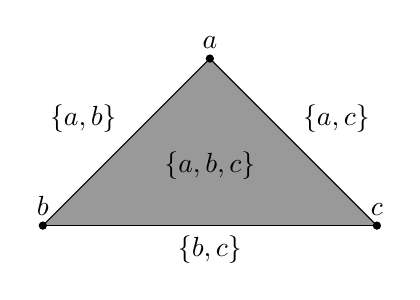
\begin{tikzpicture}[
  node distance=3cm
]
	\begin{scope}[canvas is xy plane at z=0]
		\node (a) {};
		\node (b) [below left of=a] {};
		\node (c) [below right of=a] {};

		\foreach \point in {a,b,c} 
			\fill (\point) circle(1.5pt) node[above] {$\point$};
		\foreach \linestart/\lineend/\nodepos in {a/b/above left, b/c/below, a/c/above right}
			\draw (\linestart.center) -- node[\nodepos] { \linelabel{\linestart}{\lineend} } (\lineend.center);

		\foreach \first/\second/\third in {a/b/c}
			\fill[opacity=0.4] (\first.center) -- (\second.center) -- (\third.center) (current path bounding box.center) node[below, opacity=1.0] {$\{\first,\second, \third\}$};
	\end{scope}
	% \begin{scope}{canvas is xy plane at z=4}
	% 	\node (d) {};
	% 	\fill (d) circle(1.5pt) node[above] {$d$};
	% \end{scope}
	% \draw (abc) node {$\{a,b,c\}$}
	% \draw
	% 	(0, 0) node (a0) {} node[left] {$a$}
	% 	-- node[above left] {$\{a,b\}$}
	% 	(-2, -2) node (b0) {} node[left] {$b$}
	% 	-- node[below] {$\{b,c\}$}
	% 	(2, -2) node (c0) {} node[right] {$c$}
	% 	-- node[above right] {$\{a, c\}$}
	% 	(0, 0);

	% \fill
	% 	(a0) circle(1.5pt)
	% 	(b0) circle(1.5pt)
	% 	(c0) circle(1.5pt);
	% \fill[opacity=0.4] (0,0) -- (-2, -2) -- (2, -2) -- (0,0);
\end{tikzpicture}
\end{document}
